\textbf{Consider again the approximation of $f(x)=3/(5−4cos(x))$, $x\in[-\pi,\pi]$. Let $N$ be the number of nodes in Fourier and polynomial interpolation of this function.
\begin{enumerate}[label=\alph*)]
\item Plot the error as a function of $N$ (on the same figure) for both Chebyshev and Fourier. Notice
that Fourier converges at a faster rate in this case.
\item Now consider that maximum spacing between nodes: $h=max|x_{i+1}-x_i|$. Plot the error for
polynomial and Fourier approximations as a function of $h$ and notice that the rates of convergence
are now nearly the same.
\item Show that the ratio $h_{cheb}/h_{Fourier}$ is about $\pi/2$.
\end{enumerate}
$~$}
\newline

\begin{figure}[H]
\centering
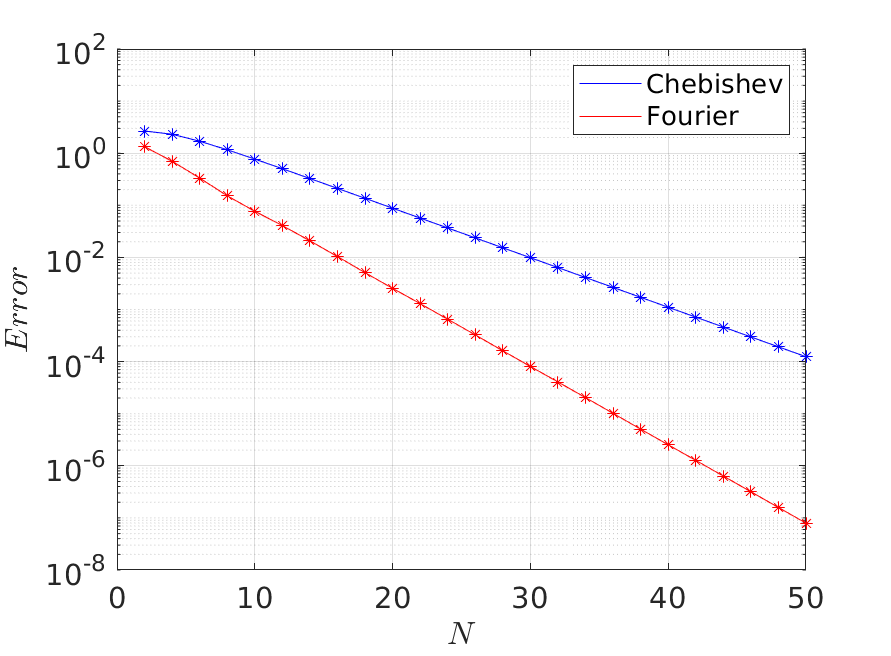
\includegraphics[scale=0.75]{P7_a.png}\caption{Convergence as $n\rightarrow\infty$ of the Chebyshev interpolant to $f(x)= \frac{\log(\frac{x+3}{4})}{x-1}$.}
\end{figure}

\begin{figure}[H]
\centering
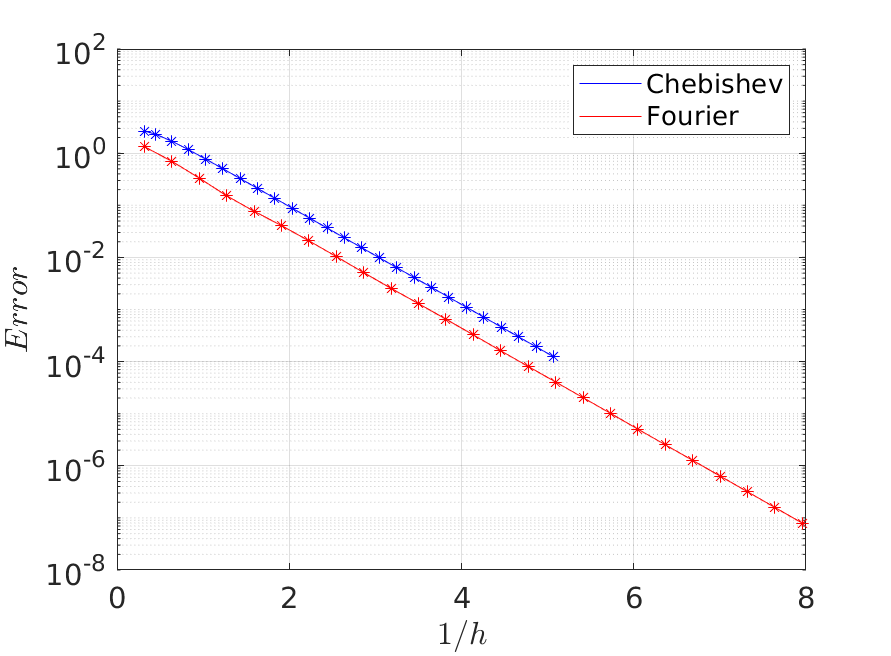
\includegraphics[scale=0.75]{P7_b.png}\caption{Convergence as $n\rightarrow\infty$ of the Chebyshev interpolant to $f(x)= \frac{\log(\frac{x+3}{4})}{x-1}$.}
\end{figure}





\subsection*{Matlab code for this problem}
\begin{verbatim}

\end{verbatim}